% Fig. 2: graph-contribution assessment protocol (standalone). Build: pdflatex -output-directory ../figures fig2_protocol.tex
\documentclass[12pt,border=3pt]{standalone}
\usepackage{lmodern}
\usepackage{amsmath}
\usepackage{tikz}
\usetikzlibrary{positioning,arrows.meta,fit,shapes.geometric}
\begin{document}
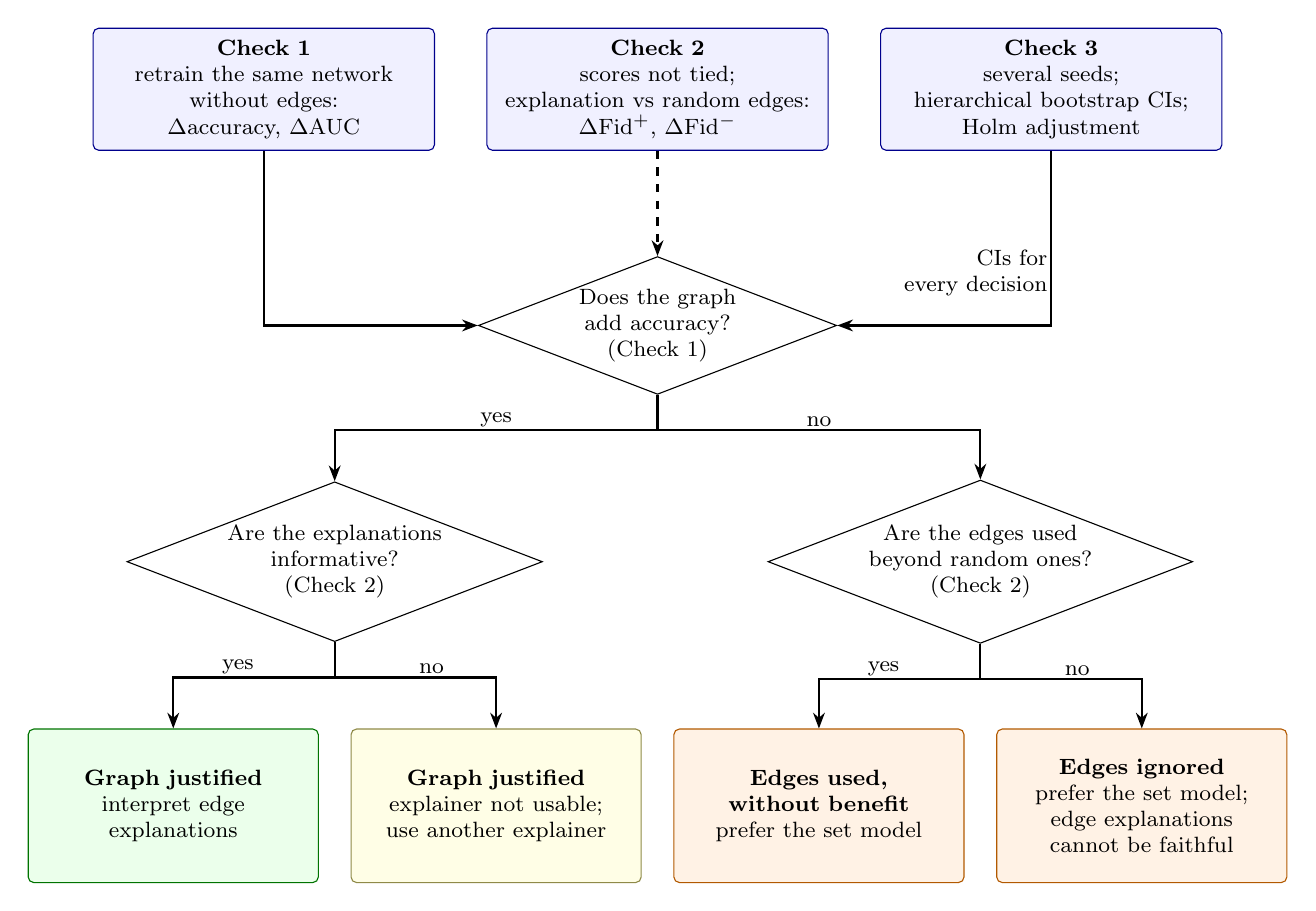
\begin{tikzpicture}[
  chk/.style={draw, rounded corners=2pt, align=center, font=\footnotesize, text width=4.1cm, minimum height=1.55cm, fill=blue!6, draw=blue!55!black},
  dec/.style={draw, diamond, aspect=2.6, align=center, font=\footnotesize, inner sep=0.5pt, fill=white},
  res/.style={draw, rounded corners=2pt, align=center, font=\footnotesize, text width=3.45cm, minimum height=1.95cm},
  arr/.style={-{Stealth[length=2mm]}, thick},
  lab/.style={font=\footnotesize, fill=white, inner sep=1pt}]
% checks
\node[chk] (c1) at (-5.0,0) {\textbf{Check 1}\\retrain the same network\\without edges:\\$\Delta$accuracy, $\Delta$AUC};
\node[chk] (c2) at (0,0) {\textbf{Check 2}\\scores not tied;\\explanation vs random edges:\\$\Delta\mathrm{Fid}^{+}$, $\Delta\mathrm{Fid}^{-}$};
\node[chk] (c3) at (5.0,0) {\textbf{Check 3}\\several seeds;\\hierarchical bootstrap CIs;\\Holm adjustment};
% decisions
\node[dec] (d1) at (0,-3.0) {Does the graph\\add accuracy?\\(Check 1)};
\node[dec] (dy) at (-4.1,-6.0) {Are the explanations\\informative?\\(Check 2)};
\node[dec] (dn) at (4.1,-6.0) {Are the edges used\\beyond random ones?\\(Check 2)};
% outcomes
\node[res, fill=green!8, draw=green!45!black] (o1) at (-6.15,-9.1) {\textbf{Graph justified}\\interpret edge\\explanations};
\node[res, fill=yellow!10, draw=yellow!50!black] (o2) at (-2.05,-9.1) {\textbf{Graph justified}\\explainer not usable;\\use another explainer};
\node[res, fill=orange!10, draw=orange!70!black] (o3) at (2.05,-9.1) {\textbf{Edges used,}\\\textbf{without benefit}\\prefer the set model};
\node[res, fill=orange!10, draw=orange!70!black] (o4) at (6.15,-9.1) {\textbf{Edges ignored}\\prefer the set model;\\edge explanations\\cannot be faithful};
% arrows from checks
\draw[arr] (c1.south) |- (d1.west);
\draw[arr, dashed] (c2.south) -- (d1.north);
\draw[arr] (c3.south) |- node[lab, pos=0.35, left, align=right] {CIs for\\every decision} (d1.east);
% decision branches
\draw[arr] (d1.south) -- ++(0,-0.45) -| node[lab, pos=0.25, above] {yes} (dy.north);
\draw[arr] (d1.south) -- ++(0,-0.45) -| node[lab, pos=0.25, above] {no} (dn.north);
\draw[arr] (dy.south) -- ++(0,-0.45) -| node[lab, pos=0.3, above] {yes} (o1.north);
\draw[arr] (dy.south) -- ++(0,-0.45) -| node[lab, pos=0.3, above] {no} (o2.north);
\draw[arr] (dn.south) -- ++(0,-0.45) -| node[lab, pos=0.3, above] {yes} (o3.north);
\draw[arr] (dn.south) -- ++(0,-0.45) -| node[lab, pos=0.3, above] {no} (o4.north);
\end{tikzpicture}
\end{document}
